\subsubsection{Performance Testservice}

Der Performance Testservice ist der Dienst, dessen Rolle die
Durchführung von Performancetests ist. Er besteht im Wesentlichen
aus zwei Containern:

\begin{itemize}
    \setlength\itemsep{1em}

    \item[] \textbf{JMeter-old und JMeter-New}: Diese beiden Container enthalten jeweils
    die jMeter-Skripte für \Gls{jexam_2009} und \Gls{jexam_new}. Die
    jMeter-Skripte wurden für beide Plattformen angepasst, da sie
    mehrere unterschiedliche Endpunkte haben.

\end{itemize}

\begin{figure}[H]
    \centering
    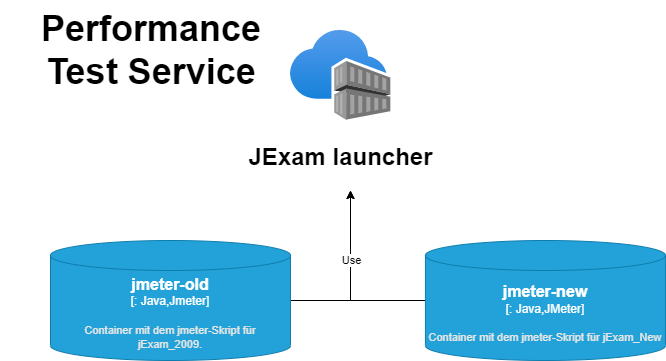
\includegraphics[scale=0.6]{images/performance.drawio}
    \caption{JExam Performance Testservice} \label{fig:per}
\end{figure}